\graphicspath{{./ch_adptv_msmnt_magnetometry_SI/figures/}}

\chapter[Adaptive sensing protocols]{Adaptive sensing protocols}
\label{ch:AMMappendix}

\section{Comparison of sensing protocols: numerical simulations}
\label{sec:comparisonprotocols}
In the following, the performances of different single-qubit frequency estimation protocols will be compared through numerical simulations. We will describe and analyse three main sensing algorithms, defined using a pseudo-code in Fig. \ref{fig:ammA1} and Fig. \ref{fig:ammA2}: the limited-adaptive, non-adaptive and optimized-adaptive protocols.

In order to achieve high dynamic range, each estimation sequence consists of \textit{N} different sensing times, multiples of the shortest sensing time $\tau_{min}$ = 20 ns: $\tau_n = 2^{N-n}$ $\tau_{min}$ (n = 1 .. \textit{N}).

After each Ramsey, the electron spin is measured: the result of each detection is indicated in the pseudo-code by the \textbf{Ramsey ($\vartheta$, $\tau$) }function. The input parameters of this function are the sensing time $\tau$ and the phase $\vartheta$ of the second $\pi$/2 pulse. In the simulation code, this function generates a random value $\mu$ ($\mu$ = 0,1), using the python library \textit{numpy.random}, chosen according to the probability distribution [$p_0$, $p_1$ = 1 - $p_0$], where:

\begin{equation}
p_0 = P(0|f_B) = \frac{1+F_0-F_1}{2}+\frac{F_0+F_1-1}{2}e^{-(\frac{\tau}{T_2^*})^2} \cos{[2\pi f_B \tau + \vartheta]}
\end{equation}

$F_0$,$F_1$  are, respectively the readout fidelities for $m_s = 0$ and $m_s = 1$. In the following simulations we use the values: $F_0$ = 0, 0.75, 0.88 or 1.00 ($m_s = 0$), $F_1$  = 0.993 ($m_s$ = 1), $T_2^*$ = 5 $\mu$s  or 96 $\mu$s.

For each Ramsey experiment (indexed here by the label $\ell$), the detection result $\mu_{\ell}$  is used to update the estimation of the magnetic field using Bayes rule: $P(f_B|\mu_1... \mu_{\ell}) \sim P(f_B|\mu_1...\mu_{\ell -1}) P(\mu_{\ell}|f_B)$. This is indicated in the pseudo-code by the function \textbf{Bayesian\textunderscore update (res, $\vartheta$, $\tau$)}.
Due to its periodicity it is convenient to express P($f_B$) in a Fourier series, resulting in the following update rule:

\begin{eqnarray}
p_k^{(\ell)} &=& \frac{1 + (-1)^{\mu_{\ell}}(F_0-F_1)}{2}p_k^{(\ell-1)}\\
\nonumber
& &+e^{-(\frac{\tau}{T_2^*})^2} \frac{(F_0+F_1)-1}{4}[e^{i(\mu_{\ell}\pi+\vartheta_{\ell})}p^{\ell-1}_{k-2^{N-n}}+e^{-i(\mu_{\ell}\pi+\vartheta_{\ell})}p^{\ell-1}_{k+2^{N-n}}]
\end{eqnarray}


Given the periodic nature of phase, the uncertainty is better estimated using the Holevo variance $V_H = (|<e^{i 2 \pi f_B \tau_{min}} >|)^{-2}-1 = ( 2 \pi|p_{(2^{N-n+1}}^{(l-1)} |)^{-2}-1$. The Holevo variance can be minimized by choosing the controlled phase \cite{Cappellaro_Phys.Rev.A_2012}:

\begin{equation}
\vartheta^{ctrl} = \frac{1}{2}\arg\{ p_{2^{N-\ell+1}}^{(\ell - 1)}\}
\end{equation}

One Ramsey experiment per sensing time does not allow to reach the Heisenberg-like scaling since the resulting probability distribution, despite being strongly peaked around the expected value, has very large wings with non-zero probability of outlier outcomes. Outliers, although occurring infrequently, can significantly alter the estimate statistics. While this is true for perfect readout ($F_0$ = $F_1$ = 1) the algorithm performance is  reduced even further by imperfect readout \cite{Said_Phys.Rev.B_2011}. A solution to these problems is to perform $M_n$ Ramsey measurements for each interaction time\cite{Said_Phys.Rev.B_2011}, with $M_n = G + F(n-1)$. 
\begin{figure*}
	\centering
	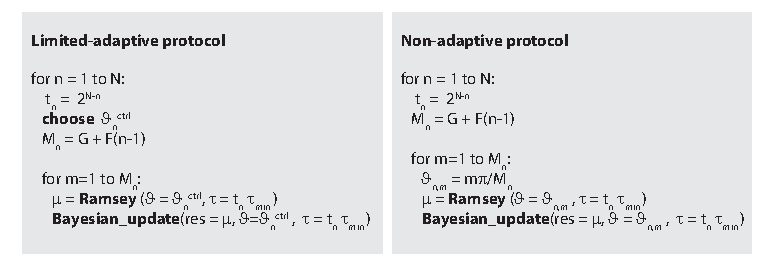
\includegraphics[width=12cm]{algorithms_1}
	\caption{\label{fig:ammA1} \textbf{Pseudo-code for the non-adaptive and limited-adaptive protocols.}}
\end{figure*}

For each protocol it is crucial to find the optimal values for \textit{F} and \textit{G}, given the experimental readout fidelities $F_0$ and $F_1$. The relevant figure of merit is the sensitivity $\eta$, defined as $\eta^2 = V_H T$.
Simulations are performed by running the protocol for 315 different values of the frequency $f_B$, over 315 repetitions for each value. The detection phase $\vartheta$ of the Ramsey is initially set to zero.

\begin{figure*}
	\centering
	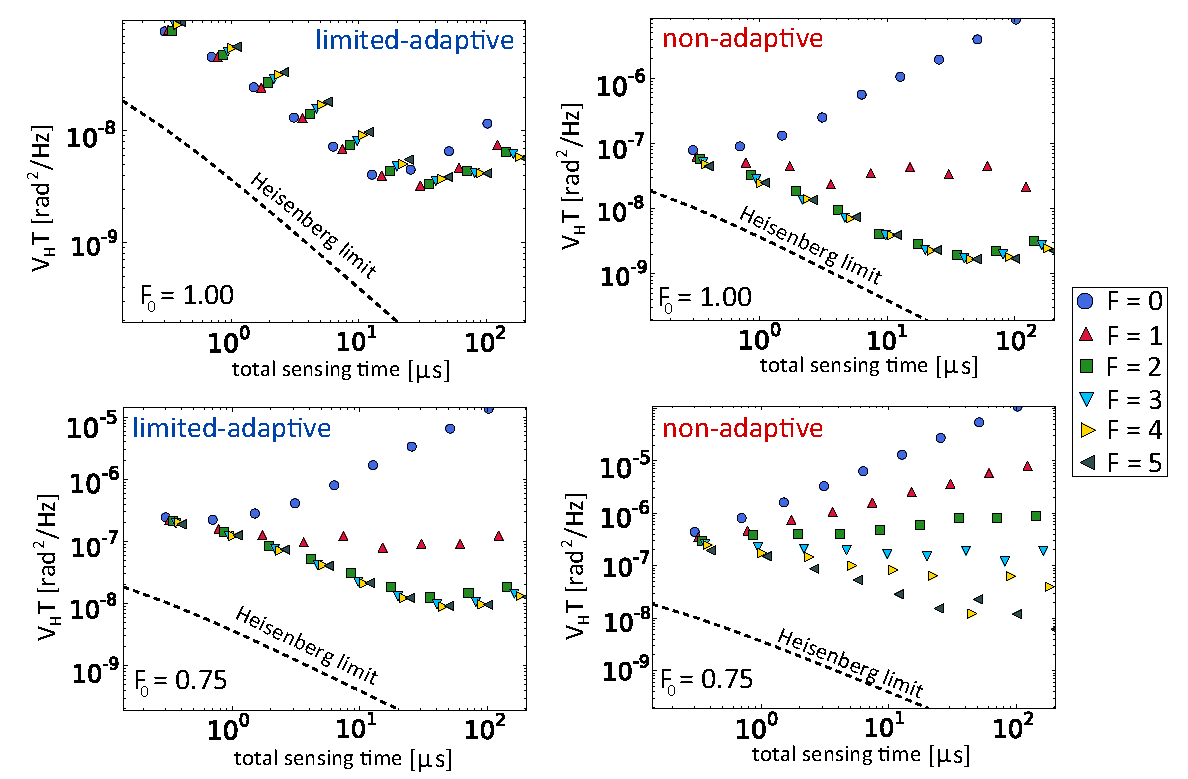
\includegraphics[width=12cm]{fig_S1}
	\caption{\label{fig:ammS1} \textbf{Non-adaptive vs limited-adaptive protocol}. Simulations comparing the limited-adaptive and non-adaptive protocols for $G = 5$, for different values of $F$, with $T_2^* = 5\mu$s. On the top row, perfect readout fidelity ($F_0 = 1$), on the bottom row, $F_0 = 0.75$. The shaded areas correspond to uncertainties (one standard deviation, calculated by a bootstrap technique). Note that the sensitivity is not further improved after the limit of $T_2^*$  is reached (total sensing time $T \sim 10\mu$s).
	}
\end{figure*}

\subsection{Limited-adaptive vs non-adaptive protocols.} 
The limited-adaptive protocol \cite{Cappellaro_Phys.Rev.A_2012} is described by the pseudo-code in Fig. \ref{fig:ammA1} (left). The controlled phase $\vartheta^{ctrl}$ is updated every time the sensing time is changed. 
In this section, the performance of the limited-adaptive protocol will be compared to the non-adaptive protocol described by Said et al. \cite{Said_Phys.Rev.B_2011} and demonstrated experimentally by Waldherr et al. \cite{Waldherr_NatNano_2012} and Nusran et al. \cite{Nusran_NatNano_2012}. The pseudo-code for the non-adaptive protocol is reported in Fig. \ref{fig:ammA1} (right). In this case, the phase of the Ramsey experiment is not updated in real-time based on the estimation of magnetic field given by the previous measurement outcomes, but its value is swept between 0 and $\pi$ according to predefined values. If, for a given sensing time, $M_n$ Ramsey experiments are performed, the Ramsey phase is increased at each step by $\pi$/$M_n$.


A comparison of the sensitivity as a function of sensing time \textit{T} for different values of \textit{F} (fixing \textit{G} = 5) is shown in \ref{fig:ammS1}. The data-points correspond to estimation sequences with increasing \textit{N} (\textit{N=} 2..10). The total sensing time \textit{T}, for each estimation sequence, is calculated as:

\begin{equation}
T=\tau_{min}[G(2^N -1)+ F(2^N - N - 1)]
\end{equation}

In top row of \ref{fig:ammS1} the sensitivities for the adaptive and non-adaptive protocols are compared in the case of perfect readout fidelities. In this case, the adaptive protocol follows a Heisenberg-like scaling already for \textit{F} = 0, even though the minimum sensitivity can only be reached for \textit{F} = 1. On the other hand, the non-adaptive protocol requires at least \textit{F} = 2 to reach Heisenberg-like scaling. On the bottom row, we compare the sensitivities for reduced readout fidelity ($F_0$ = 0.75). Here, the adaptive protocol reaches HL-scaling for $F\geq2$, while the non-adaptive protocol can only get close to it with $F=5$. 
It is important to stress that, in both cases, there is a big improvement when $M_n$ is a function of $n$ ($F>0$) compared to the case where $M_n$ is independent of $n$ ($F=0$). In other words, it is beneficial to repeat more often Ramsey experiments with shorter sensing time. The reason is two-fold: on one end they contribute less to the total sensing time, on the other end they are related to larger frequencies which, if estimated wrong, would give a larger error.

\begin{figure*}
	\centering
	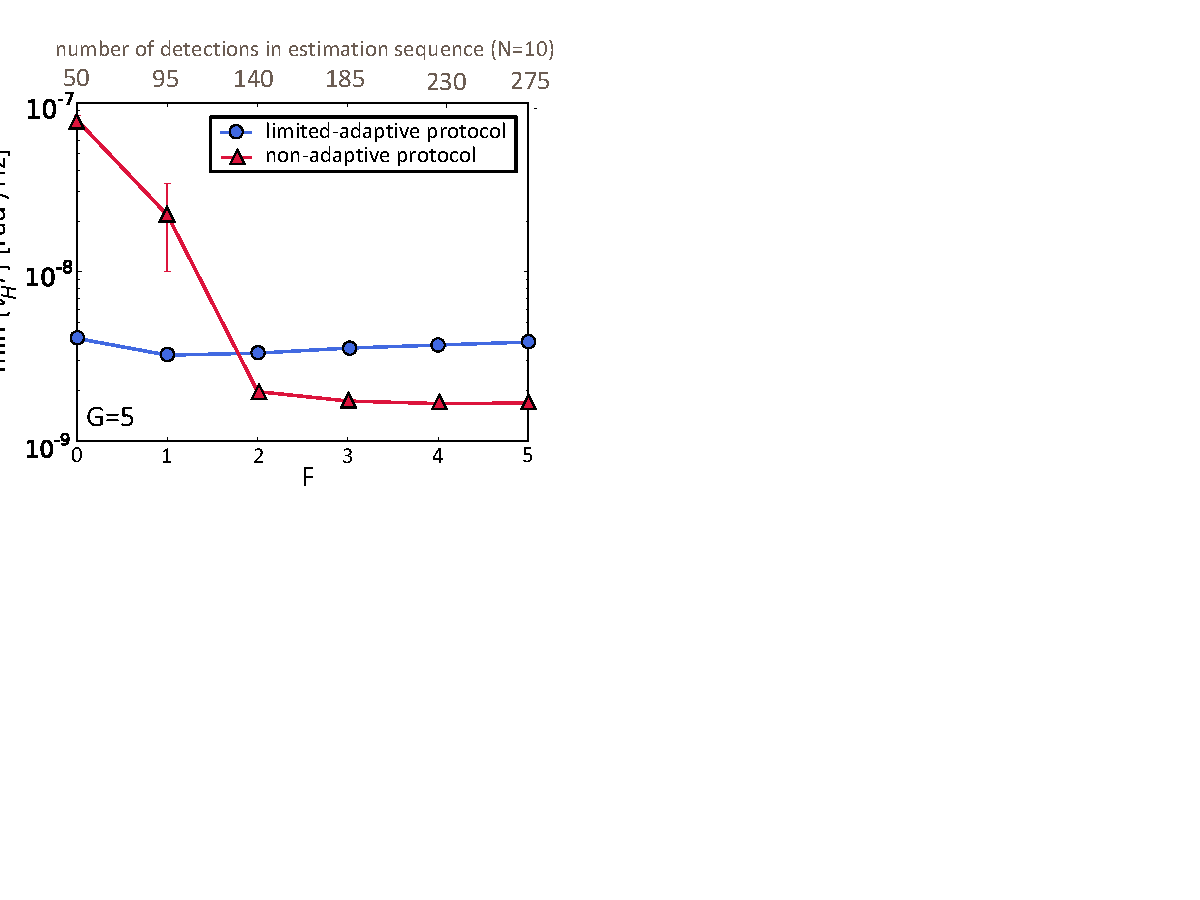
\includegraphics[width=6cm]{fig_S2}
	\caption{\label{fig:ammS2} \textbf{Simulation results for the best achieved sensitivity, comparing the limited-adaptive and non-adaptive protocols as a function of F}. Here, we assume perfect readout fidelity ($F_0=1$) and $T_2^* = 5\mu$s. On the top x-axis, the total number of Ramsey experiments in the estimation sequence for $N = 10$ is reported. Error bars, corresponding to one standard deviation, are calculated by bootstrap.
	}
\end{figure*}

Comparison between protocols is easier when plotting only the minimum sensitivity vs $F$. This is shown in Fig. \ref{fig:ammS2} for perfect readout fidelity $F_0=1$. We find that for $F<2$, the limited-adaptive protocol outperforms the non-adaptive protocol. This is expected since in this region only the limited-adaptive protocol exhibits Heisenberg-like scaling. However, once the non-adaptive protocol achieves Heisenberg-like scaling ($F\geq2$) it reaches a lower sensitivity.

On the scale at the top of Fig. \ref{fig:ammS2}, the number of Ramsey runs corresponding to an estimation sequence with $N = 10$ different sensing times is reported. By increasing $F$, the number of Ramsey experiments increases as:

\begin{equation}
R_N = GN + \frac{FN(N-1)}{2}
\end{equation}

For perfect readout fidelity, the limited-adaptive protocol reaches HL-scaling for $F=0$: therefore it only requires $R_N = 50$ Ramsey runs in the estimation sequence. On the other hand, the non-adaptive requires $F=2$, i.e. $R_N = 140$ Ramsey runs. Each Ramsey comprises an initialization/measurement duration, labelled as `overhead', not included in the plots (where we only take the sensing time into account). In practice, it is however necessary to minimize the total time of the sequence (including overhead), so that protocols that achieve Heisenberg-like-scaling with smaller $F$ (and therefore less detections $R_N$) are to be preferred as discussed in the main text (Fig. \ref{fig:amm-fig5}).


A striking result is the fact that once the non-adaptive protocol reaches Heisenberg-like-scaling it achieves a better sensitivity than the limited-adaptive one. Since non-adaptive protocols are a particular case of the most general class of adaptive protocols, this indicates that the limited-adaptive protocol is not optimal and that protocols with better performance must exist.

\subsection{Optimized adaptive protocol. }
\begin{figure*}[h!]
	\centering
	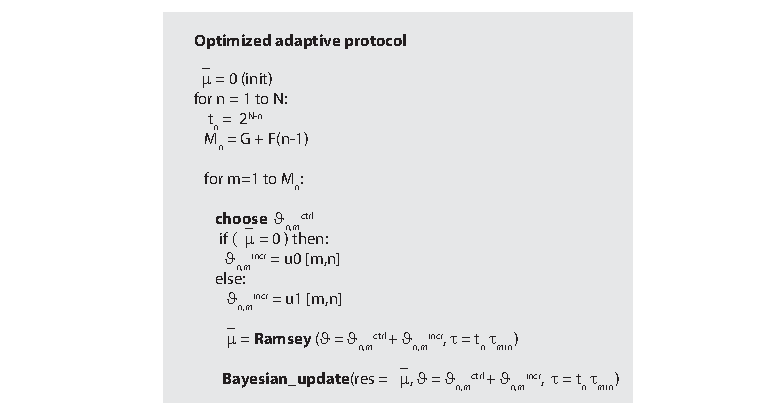
\includegraphics{algorithms_2}
	\caption{\label{fig:ammA2} \textbf{Pseudo-code for the optimized adaptive protocol.}}
\end{figure*}
In order to improve the performance of the limited-adaptive protocol, we consider two modifications:\\

Firstly, the controlled phase is estimated not only when changing sensing time, but before each Ramsey measurement (\textit{full-adaptive} protocol). The improvement achieved with this modification can be observed in Fig. \ref{fig:ammS3}, where we compare simulations for controlled phase updated only when changing sensing time and before each Ramsey. In the left plot, we compare the sensitivity, for increasing number of measurements $N$ ($N=2..10$) in the case ($G=3$,$F=0$). Both protocols scale better than the standard quantum limit only for the first few data-points (until $N>4$). However, the absolute sensitivity of the full-adaptive protocol is a factor two better. In the central plot, the same curves are displayed for ($G=3$,$F=5$). For these parameters, Heisenberg-like scaling is maintained until the coherence time limit is reached. Again, the full-adaptive protocol is better than the limited-adaptive for all $N$. In the right plot, we show the minimum achieved sensitivity for both protocols, as a function of $F$. In all cases the full-adaptive protocol outperforms the protocol which updates the optimal phase only when changing the sensing time. Additional simulations (not shown) for different values of $G$, or imperfect readout fidelity, confirm the improvements gained by the full-adaptive strategy. \\
\begin{figure*}
	\centering
	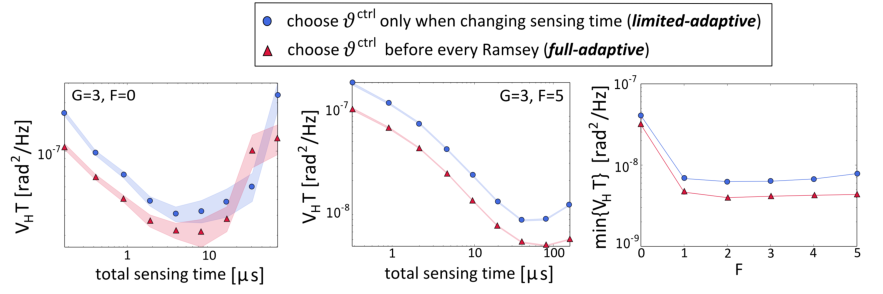
\includegraphics[width=12cm]{fig_S3_new}
	\caption{\label{fig:ammS3} \textbf{Comparison adaptive protocols} Adaptive protocols: simulation results comparing sensitivities obtained when updating the controlled phase only when changing sensing time (blue) and updating it before each Ramsey (red). We assume perfect readout fidelity and $T_2^* = 5\mu$s. Shaded areas represent error bars corresponding to one standard deviation (bootstrap method). 
	}
\end{figure*}
The second modification was suggested by A. J. Hayes and D. W. Berry \cite{Hayes_Phys.Rev.A_2014}. They proposed a protocol where the detection phase of the Ramsey experiment is $\vartheta_{(n,m)} = \vartheta_{(n,m)}^{ctrl} + \vartheta_{(n,m)}^{incr}$. A phase increment $\vartheta_{(n,m)}^{incr}$, dependent only on the last measurement outcome, is added to the controlled phase $\vartheta_{(n,m)}^{ctrl}$. The phase increment is obtained by numerically optimizing the final variance in frequency estimation for the specific experimental parameters through a \textit{swarm optimization} procedure\cite{Hayes_Phys.Rev.A_2014,Hentschel_Phys.Rev.Lett._2010,Bratton__2007}. In the pseudo-code this step is represented by the functions u0, u1. \\

The optimized adaptive protocol, described in Fig. \ref{fig:ammA2}, combines phase increments with update of the controlled phase before each Ramsey. A comparison between the minimum sensitivity achieved by the limited-adaptive, non-adaptive and optimized-adaptive protocols is reported in Fig. \ref{fig:ammS4}. The optimized adaptive protocol appears to perform always at least as good as the best between the limited-adaptive and the non-adaptive protocols. For lower values of $F$, the non-adaptive protocol fails to reach HL-scaling, while both adaptive ones do. For higher values of $F$, both the non-adaptive and the optimized adaptive reach the minimum sensitivity. Note that, for a readout fidelity $F_0 = 0.88$, while the optimized adaptive protocol reaches HL-scaling for ($G = 5$,$F = 2$) the non-adaptive one needs at least $F = 4$.


\begin{figure*}
	\centering
	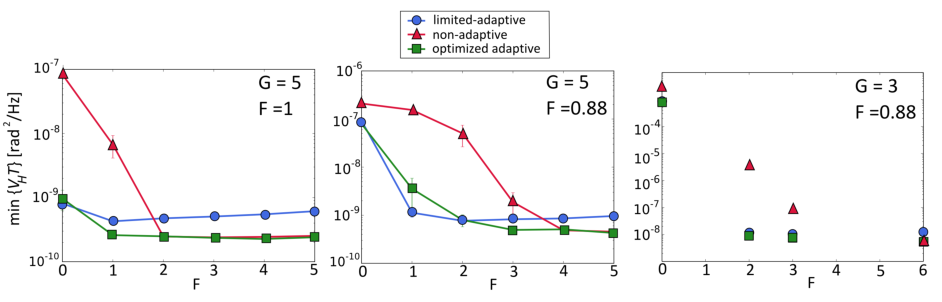
\includegraphics[width=12cm]{fig_S4_new}
	\caption{\label{fig:ammS4} \textbf{Comparing all protocols.} Simulations comparing the best achieved phase sensitivities for different protocols ($G = 5$ left and central plots, $G = 3$ for the plot on the right). We assume $T_2^* = 96\mu$s. The optimized adaptive protocol performs always at least as well as the non-adaptive protocol. For a fixed value of $G$, the optimized adaptive protocol reaches the best sensitivity for a smaller value of $F$.
	}
\end{figure*}
\section{Application to room-temperature sensing.}
\label{sec:ammSIRTsens}
\begin{figure*}
	\centering
	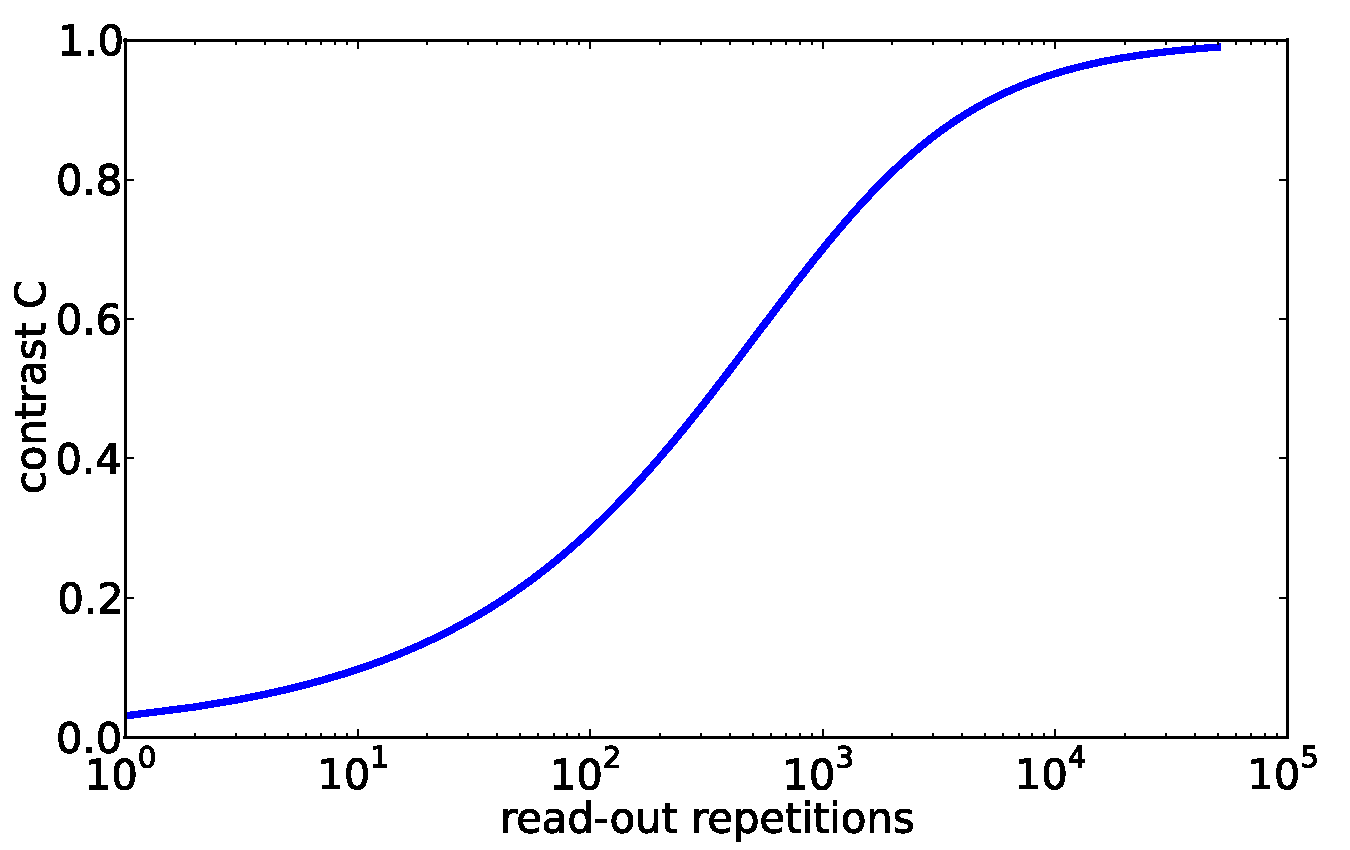
\includegraphics[width=6cm]{fig_S5}
	\caption{\label{fig:ammS5} \textbf{Contrast for room-temperature readout} Effective readout fidelity as a function of readout repetitions, for measurements at room-temperature (no single-shot readout).
	}
\end{figure*}

At room-temperature, the spin-selective optical transitions within the zero-phonon line are not spectrally-resolvable and therefore single-shot spin initialization and readout by resonant optical excitation is not possible. Instead, the readout exploits the small difference in luminescence intensity by off-resonant optical excitation (in the green) when the electron spin is in $m_s = 0$, compared to $m_s = 1$. In the following, we will use numbers from Nusran et al. \cite{Nusran_NatNano_2012}, that report $\alpha_0 = 0.031$ photons per shot when the electron is in $m_s = 0$, $\alpha_1 = 0.021$ photons per shot when the electron is in $m_s = 1$.  Since one shot is not enough to perfectly distinguish between the two states, room-temperature experiments are repeated $R$ times. The resulting signal level is then, respectively, $\alpha_0 R$ and $\alpha_1 R$. The contrast $C$ for a single repetition scales as \cite{Taylor_NatPhys_2008}:

\begin{equation}
\frac{1}{C} = \sqrt{1+\frac{2(\alpha_0 + \alpha_1)}{(\alpha_0-\alpha_1)^2R}}
\end{equation}

\begin{figure*}
	\centering
	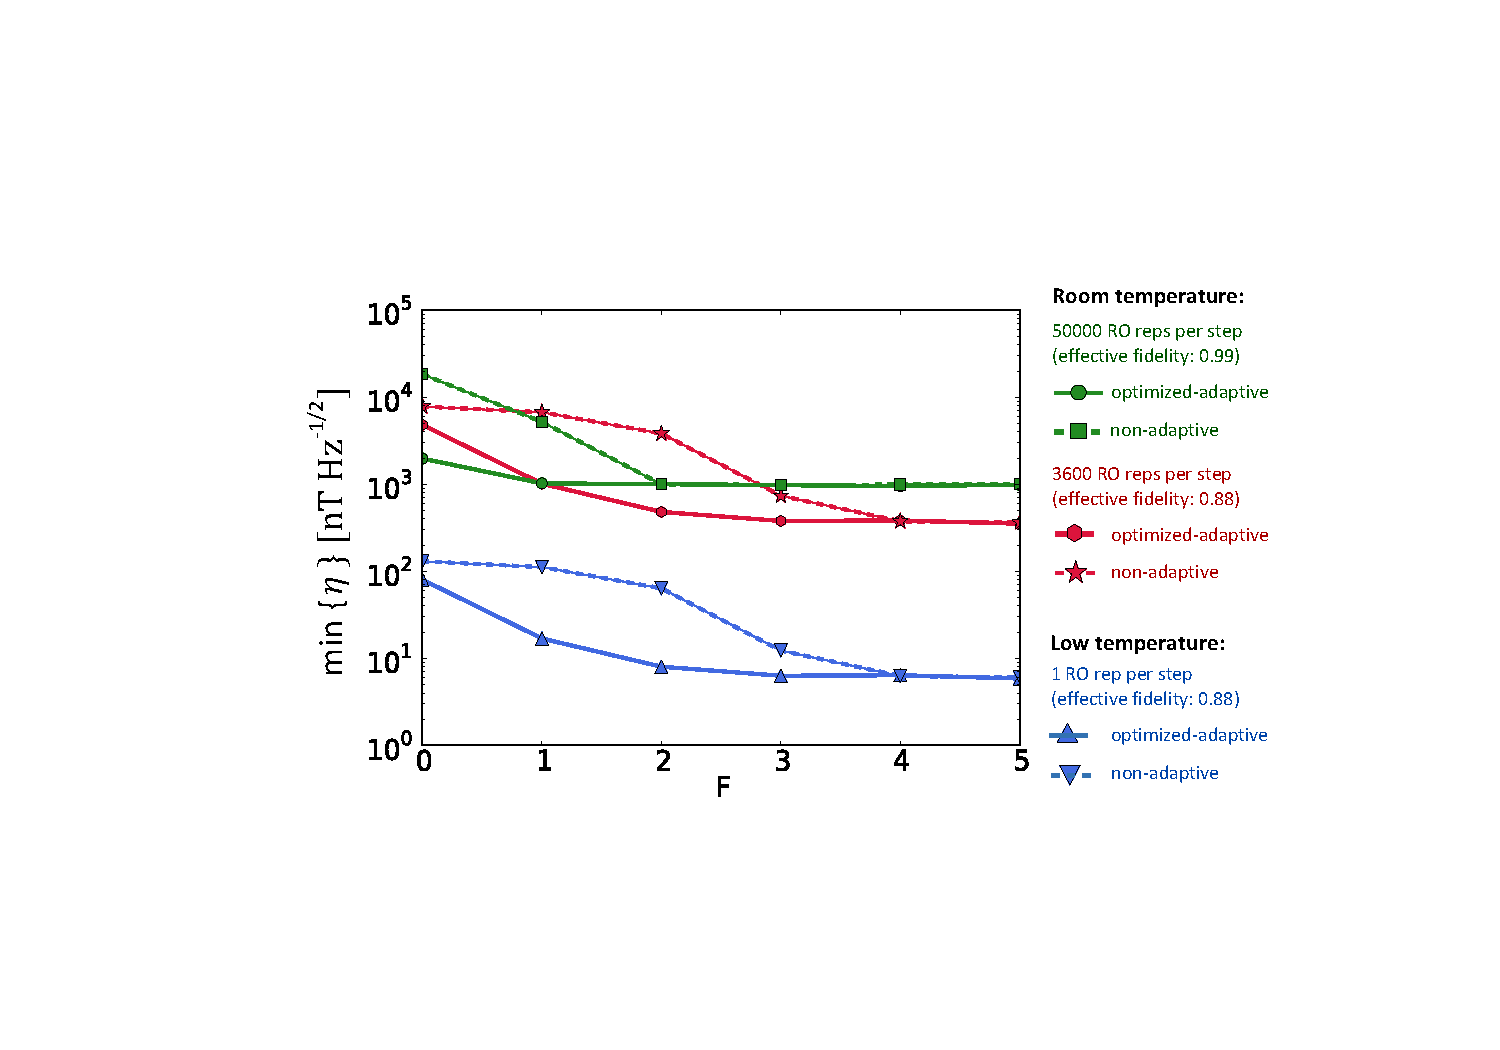
\includegraphics[width=12cm]{fig_S6}
	\caption{\label{fig:ammS6} \textbf{Adaptive protocol for room-temperature} Simulations comparing the minimum magnetic field sensitivity (in nT Hz$^{-\frac{1}{2}}$) for the optimized adaptive and the non-adaptive protocols at room-temperature and low-temperature ($T_2^* = 96 \mu$s, $N = 10$, $G = 5$). 
	}
\end{figure*}
This contrast $C$ is related to the fidelity with which the two states can be distinguished and, since luminescence detection is shot-noise limited, the error scales at the standard quantum limit as $R^{-\frac{1}{2}}$. Nusran et al. achieve a fidelity of 0.99, in their experiment \cite{Nusran_NatNano_2012}, by using 50000 readout repetitions per step. The achieved contrast as a function of readout repetitions is plotted in Fig \ref{fig:ammS5}.
A contrast $C = 0.75$ can be achieved with $R = 1350$ repetitions, while $R = 3600$ repetitions are needed for $C = 0.88$, significantly less than the repetitions (50000) needed for almost perfect readout ($C = 0.99$). 
In the simulations in Fig. \ref{fig:ammS6}, for consistency with previous results, we assume asymmetric readout fidelity ($F_1 = 0.993$,$F_0 = C+(1-F_1)$), based on the contrast $C$ achieved with a given number of readout repetitions. The asymmetry of the readout fidelity can be controlled at will by choosing the threshold in photo-counts distinguishing $m_s = 0$ from $m_s = 1$.

Simulation results show that, at room temperature, the use of 50000 repetitions can achieve a sensitivity of $\eta \sim 1$ $\mu$T Hz$^{-\frac{1}{2}}$, either using the adaptive or non-adaptive protocols. However, using 3600 repetitions per step (with a lower effective readout fidelity), a better sensitivity $\eta \sim 0.4$ $\mu$T Hz$^{-\frac{1}{2}}$ can be reached. Moreover, for $F = 2$, the performance of the optimized-adaptive protocol with 3600 readout repetitions per step surpasses both the performance of the non-adaptive for the same conditions and the performance of the protocols with 50000 repetitions per step. For $F \geq 4$ adaptive and non-adaptive reach the same sensitivity: however, as discussed above and in the main text, a smaller value of $F$ allows a higher repetition rate of the estimation sequence.

This suggests the possibility that adaptive sensing, which reaches Heisenberg-limited scaling for a reduced number of measurements even in situation of lower fidelity, may be advantageous for room-temperature sensing, compared to non-adaptive protocols.
Simulations confirm the superior performance of the protocol in the case where single-shot readout is available, enabling sensitivities on the order of a few nT Hz$^{-\frac{1}{2}}$, as demonstrated experimentally by the data reported in the main text.


\section{Experimental techniques}

Microwave (MW) signals to drive the NV centre electron spin are generated by a Rohde Schwarz SMB100A source, with IQ modulation.  To create the two $\pi$/2 pulses for each Ramsey experiment, the MW source output frequency is modulated (single-sideband modulation) by two pulses with rectangular envelope and 30 MHz carrier frequency. The first pulse is generated directly by an AWG (Arbitrary Waveform Generator, Tektronix AWG5014), the second by a field-programmable logic array (FPGA). The FPGA receives the value for the phase $\vartheta$ chosen by the control microprocessor (ADwin Gold) and generates the modulation pulse with the proper IQ parameters, with timing triggered by the AWG. The value for the phase $\vartheta$ is specified as an 8-bit integer (256 levels), leading to a resolution of 1.4 degrees (0.025 radians).
Due to the hyperfine coupling to the host $^{14}$N spin, the electron spin transition is split into three frequency-separated lines. As discussed in Section \ref{sec:ammMW}, these three lines are addressed separately by three Ramsey experiments, realized by driving the electron spin at the three frequencies. This is achieved by an additional frequency modulation, imposed to the vector source by the AWG. The microprocessor (Adwin Gold) manages the sequence  of control pulses (optical and microwave) and counts the luminescence photons during spin readout. Moreover, it performs the Bayesian update of the probability density distribution $P(f_B)$ and chooses the proper controlled phase and phase increments. 

\subsection{Bayesian estimation with microprocessor}
\label{ammSI:overhead}
The microprocessor code for Bayesian update minimizes the number of coefficients $p_k$ (Eq. S-E2) to be tracked and stored, to avoid exceeding the memory bounds of the microprocessor, and to optimize speed. We only use the coefficients which are known to be non-zero and contribute to the choice of the controlled phase $\vartheta$, neglecting the rest. Since the probability distribution is real ($p_k^* = p_{-k}$), we can further reduce the computational requirements by only storing the coefficients for $k>0$. Considering all this, the number of coefficients that needs to be processed, at each step $n$, is on the order of $M = G+F(n-1)$.

\begin{table}[]
\centering
\begin{tabular}{ccccc}
\hline
\multicolumn{1}{l}{\textbf{N}} & \multicolumn{1}{l}{\textbf{\begin{tabular}[c]{@{}l@{}}initialization\\ time {[}ms{]}\end{tabular}}} & \multicolumn{1}{l}{\textbf{\begin{tabular}[c]{@{}l@{}}sensing\\ time {[}ms{]}\end{tabular}}} & \multicolumn{1}{l}{\textbf{\begin{tabular}[c]{@{}l@{}}readout\\ time {[}ms{]}\end{tabular}}} & \multicolumn{1}{l}{\textbf{\begin{tabular}[c]{@{}l@{}}computational\\ time {[}ms{]}\end{tabular}}} \\ \hline
\rowcolor[HTML]{C0C0C0} 
\textbf{5}  & 9.0 & 0.004 & 1.80 & 4.0 \\
\textbf{7}  & 15.4 & 0.018 & 3.08  & 8.0  \\
\rowcolor[HTML]{C0C0C0} 
\textbf{8}  & 19.2 & 0.035 & 3.84 & 10.8  \\
\textbf{9}  & 23.4 & 0.071 & 4.68 & 13.9 \\
\rowcolor[HTML]{C0C0C0} 
\textbf{10} & 28.0 & 0.140 & 5.60  & 17.6 \\
\textbf{12} & 38.4 & 0.573 & 7.68  & 26.8  \\ \hline
\end{tabular}
\caption{\textbf{Temporal budget of the estimation protocol.} Total time, measured by the internal microprocessor clock, spent by the optimized-adaptive protocol in different tasks within the whole estimation sequence. The computational time (i.e. the time spent by the processor in performing the Bayesian update), is similar to that spent on spin initialization. Given that initialization and Bayesian update can be performed simultaneously, the computational time represents no additional overhead. }
\label{tab:ammtable_overhead}
\end{table}
In the case ($G = 5$, $F = 2$), the time spent by the microprocessor in the Bayesian update after each Ramsey experiment increases linearly from 80 $\mu$s (for $n = 2$) to 190 $\mu$s (for $n = 12$). This time is comparable with the spin initialization duration (200 $\mu$s). In Table \ref{tab:ammtable_overhead} we show the total times associated with sensing, initialization, and computation of the Bayesian estimate. While in this work we performed the initialization and the Bayesian estimate sequentially, both operations can be performed simultaneously. In this way the real-time Bayesian estimation, a crucial prerequisite for the adaptive technique, does not add any temporal overhead to the protocol. In future implementations, the Bayesian estimation could be implemented with a dedicated FPGA, instead of a general-purpose microprocessor, which would allow a further reduction of the calculation time.

\subsection{Microwave pulses and coupling to the $^{14}$N spin}
\label{sec:ammMW}
When using the electron spin of the NV center as a sensor in a Ramsey interferometry experiment, the coupling to its host $^{14}$N nuclear spin has to be taken into account. The hyperfine interaction ($\hat{H}_{hf}=A_{hf} \hat{S}_z \hat{I}_z$, neglecting small off-diagonal terms) effectively splits the electron spin $m_s = 0 $ to $m_s = -1$ transition in three lines (Fig. \ref{fig:ammS7}b).  Although these three lines can be addressed simultaneously by selecting a Rabi frequency larger than the coupling strength, the phase acquired during free evolution will depend on the state of the $^{14}$N spin. This creates ambiguity in the frequency estimation protocol, since the aim is to sense only the change in energy levels introduced by the Zeeman shift induced by the applied magnetic field, not the coupling to the $^{14}$N spin.

To circumvent this problem, we perform three sequential Ramsey sequences where, in each sequence, the microwave pulses are resonant with one of the three $m_s = 0$ to $m_s = -1$ transitions and the acquired phase only depends on the Zeeman shift. We choose the Rabi frequency (140 kHz) such that the pulses in each sequence only address selectively one of the three transitions. In Fig. \ref{fig:ammS7}, we show that we can perform Rabi oscillations selectively on the Nitrogen spin. Here the microwave pulses only drive the electron spin $m_s = 0$ to $m_s = -1$ transition if they are on resonance, thus for the $^{14}$N spin in a mixed state, a contrast of 1/3 is expected. Full contrast is recovered when the three pulses are applied sequentially (Fig. \ref{fig:ammS7}c).

\begin{figure*}
	\centering
	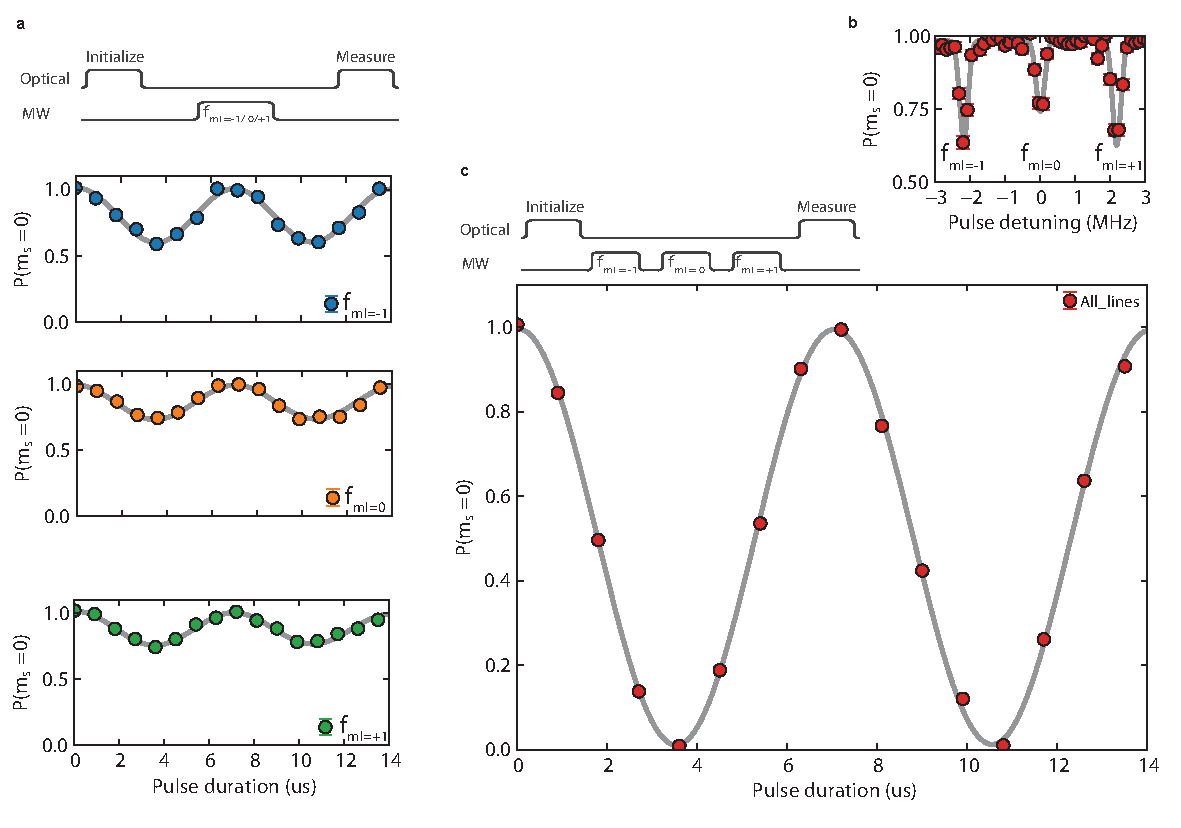
\includegraphics[width=12cm]{Rabi_diff_hf_lines}
	\caption{\label{fig:ammS7} \textbf{Electron spin driving.} a) Rabi oscillations of the electron spin conditional on the state of the  nitrogen spin ($^{14}$N , $I = 1$). We tune the frequency of the microwave pulses in resonance with one of the three $m_s = 0$ to $m_s = -1$ transitions, corresponding to the nitrogen spin being either in $m_I = -1 , 0$ or $+1$ (top, middle bottom) and vary the length of the pulse. From a sinusoidal fit (grey line) we find Rabi frequencies of  (144, 140 and 142 $\pm$ 2 kHz) respectively b) Energy level spectrum for the electron $m_s = 0$ to $m_s = -1$ transition. We initialize the electron spin in $m_s = 0$ and then vary the frequency of a microwave pulse with fixed length. The pulse detuning is with respect to a reference frequency of 2.845334 GHz.  The spectrum shows three lines owing to the hyperfine interaction with the $^{14}$N spin with $|A_{hf}| = 2\pi x (2.185  \pm 0.006)$ MHz. c) Rabi oscillation of the electron spin unconditional on the state of the nitrogen spin. We apply three sequential microwave pulses each on resonance with one of the hyperfine lines. From the sinusoidal fit (grey line) we find a Rabi frequency of $(142 \pm 3)$ kHz.}
\end{figure*}

We note that this method requires the electron transition energies and therefore the static magnetic field to be known within the bandwidth of the pulses ($\sim$ 140 kHz). This is not a problem for our implementation, where the effect of an external field is implemented as an artificial detuning by adjusting the phase of the final $\pi$/2 pulse. When estimating a real magnetic field possible solutions would be to initialize the nitrogen spin, adjust the frequency estimation protocol to allow for sensing of multiple frequencies with fixed offset or adjust the interaction times such that the phase acquired during free evolution is independent of the state of the nitrogen spin ($2 \pi = \tau A_{hf}$).

\subsection{NV charge state and optical resonance pre- and post-selection.}
Due to environmental charge noise, the optical transitions of the NV centre shift in frequency on a range larger than the linewidth. Moreover, resonant excitation can result in ionization of the NV$^-$ charged state into the neutral NV$^0$ state.
Before each estimation sequence, we check that the centre is in the NV$^-$ state, with optical transitions resonant with the excitation lasers. We turn both the initialization and readout lasers (on transitions E’ and $E_y$, respectively) for 150 $\mu$s and count luminescence photons. Only if the luminescence photo-counts are larger than a given threshold (40 counts), the estimation sequence is started (charge and optical resonance pre-selection). We take the absence of luminescence photo-counts as an indication that the centre is ionized into the NV$^0$ state: the correct charge state is restored by resonant optical excitation of the NV$^0$ transition at 575 nm.
An estimation sequence can consists of a large series of Ramsey experiments, with spin initialization and readout. Ionization of the defect or large frequency shifts of the optical transitions during the sequence results in incorrect spin readout and errors in the magnetic field estimation. Therefore, we perform a new check of the charge and optical resonance conditions at the end of the estimation sequence and consider it as a valid estimation only if more than 10 luminescence photo-counts are detected (charge and optical resonance post-selection).
In the histograms in Fig. \ref{fig:ammS8}, we report an example of the number of rejected runs for 225 repetitions of the estimation sequence. While the average number of rejections in the post-selection process is around 50\%, we have a consistent fraction of events (75/252) with no rejections, and other runs with 80\% failure rate. This large spread is due to the fact that the data was taken in long automated measurement session during nights, with infrequent optimizations of the experimental parameters (like spatial overlap of laser beams on the NV centre). We believe that the percentage of rejected runs can be drastically reduced by optimizing the experimental settings and procedures.
\begin{figure*}
	\centering
	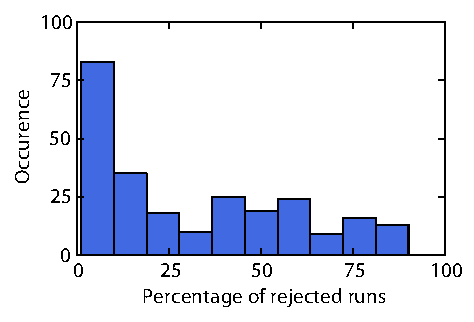
\includegraphics{Failed_CR_checks}
	\caption{\label{fig:ammS8} \textbf{Charge resonance statistics.} Histograms of the percentage of rejected runs in charge and optical resonance post-selection.}
\end{figure*}
\bibliographystyle{../thesis}
\bibliography{amm_appendix}
